
\newpage
\section{Chapter 4 - Inequalities}

\subsection*{Practical Example}
\textbf{Example 1 - Markov's Inequality}.\\
You hear that the mean age of NYU students is 20 years, but you know quite a few
students that are older than 30. You decide to apply Markov's inequality to bound
the fraction of students above 30 by modeling age as a nonnegative random variable A.
$$
\P(A > 30) \leq \frac{\E[A]}{30} = \frac{2}{3},
$$
so at most two thirds of the students are over 30.
This isn't a very precise bound, but then we also only use the expectation.

\medskip\noindent
\textbf{Example 2 - Chebyshev's Inequality}.\\
The previous bound is a little too weak. After investigating we discover that the
standard deviation of student age is actually just 3 years. Applying Chebyshev's
inequality to this information and obtain
$$
\P(|A - \E[A]| > 10) \leq \frac{\V(A)}{100} = \frac{9}{100}.
$$
So at least 91\% of the students are under 30 years old (and above 10).

\subsection*{Exercises}
%%%%%%%%%%%%%%%%%%%%%%%%%%%%%%%%%%%%%%%%%%%%%%%%%%%%%%%%%%%%%%%%%%%%%%%%%%%%%%%
\textbf{4.1}\\  % PDF page 68
Let $X\sim\text{Exp}(\beta)$. As we found in exercise 3.12, $\mu = \E[X] = \beta$ and
$\sigma^2 = \V(X) = \beta^2$. By applying Chebyshev's inequality:
$$
\P(|X-\beta|\geq t) = \P(|X-\mu|\geq t) \leq \frac{\sigma^2}{t^2} = \frac{\beta^2}{t^2}
$$
We are going to compare Chebyshev's inequality with the following inequality. Since $\sigma\geq 0$
and $k > 1$, we can apply Markov's inequality to get:
$$
\P(|X-\mu|\geq k\sigma) = \P((X-\mu)^2\geq k^2\sigma^2) \leq
\frac{\E[(X-\mu)^2]}{k^2\sigma^2} = \frac{\sigma^2}{k^2\sigma^2} = \frac{1}{k^2}
$$
We recognize this as the corollarly to the Chebyshev inequality. Comparing,
and using that $\sigma = \beta$, and using $t$ instead of $k$:
\begin{align*}
    \P(|X-\beta|\geq t) &\leq \frac{\beta^2}{t^2} \\
    \P(|X-\beta|\geq t\beta) &\leq \frac{1}{t^2}
\end{align*}
If $\beta > 1$, the first bound becomes 'weaker' which makes sense since $\beta t > t$ and
we are considering a smaller interval. If $\beta < 1$ the reverse is true. Also interesting
to note that by scaling up the bounded interval by $\beta$ gives a $\beta^2$ increase in the
bound, provided that $\beta > 1$. Shows there is a nonlinear relationship for the bound
when using the Exponential distribution.

\newpage\noindent
%%%%%%%%%%%%%%%%%%%%%%%%%%%%%%%%%%%%%%%%%%%%%%%%%%%%%%%%%%%%%%%%%%%%%%%%%%%%%%%
\textbf{4.2}\\  % PDF page 68
Let $X\sim\text{Poisson}(\lambda)$. As seen, $\E[X] = \lambda$ and
$\V(X) = \lambda$. Applying Chebyshev's inequality to show that
$\P(X\geq 2\lambda) = 1/\lambda$.
$$
\P(X \geq 2\lambda) = \P(X - \lambda \geq \lambda) \leq
\P(|X - \lambda| \geq \lambda) \leq \frac{\lambda}{\lambda^2} = \frac{1}{\lambda}.
$$
Which shows that $\P(X \geq 2\lambda) \leq 1/\lambda$.

\bigskip\noindent
%%%%%%%%%%%%%%%%%%%%%%%%%%%%%%%%%%%%%%%%%%%%%%%%%%%%%%%%%%%%%%%%%%%%%%%%%%%%%%%
\textbf{4.3}\\  % PDF page 68
Let $X_1,\ldots,X_n\sim\text{Bernoulli}(p)$ and define
$$
\bar{X} = \frac{1}{n}\sum_{i=1}^nX_i.
$$
Bound $\P(|\bar{X} - p| > \epsilon)$ with Chebyshev's and
Hoeffding's inequality. Show that when $n$ is large, the
Hoeffding's bound is smaller than Chebyshev's bound. (Assuming $\epsilon > 0)$.

For the Bernoulli distribution, $\E[X_i] = p$ and $\V(X_i) = p(1-p)$.
Since we are using a statistic, $\E[\bar{X}] = p$ and $\V(\bar{X}) = p(1-p)/n$
as per Theorem 3.17. Applying Chebyshev's inequality:
$$
\P(|\bar{X} - p| > \epsilon) \leq \frac{p(1-p)/n}{\epsilon^2} = \frac{p(1-p)}{n\epsilon^2}
\leq \frac{1/4}{n\epsilon^2} = \frac{1}{4n\epsilon^2}
$$
(Using that the max value of $p-p^2$ is 1/4 for $p\in(0,1)$).
Applying Hoeffding's inequality via Theorem 4.5.
$$
\P(|\bar{X} - p| > \epsilon) \leq 2e^{-2n\epsilon^2} = \frac{2}{e^{2n\epsilon^2}}
$$
To examine what happens as $n$ grows, we divide the Hoeffding bound by the Chebyshev bound
and call it $L_n$:
$$
L_n = 
\left(\frac{2}{e^{2n\epsilon^2}}\right)
\Big/
\left(\frac{1}{4n\epsilon^2}\right)
= \frac{8n\epsilon^2}{e^{2n\epsilon^2}}
$$
If we take the limit when $n\ra\infty$, both the numerator and denominator diverges.
So we apply L'Hôpital's rule and differentiate the numerator and denominator wrt. $n$:
$$
\lim_{n\ra\infty} L_n = 
\lim_{n\ra\infty} \frac{8n\epsilon^2}{e^{2n\epsilon^2}} = 
\lim_{n\ra\infty} \frac{8\epsilon^2}{2\epsilon^2e^{2n\epsilon^2}} = 0
$$
Since we lose the dependence on $n$ in the numerator, the fraction goes to 0 as $n$ grows.
So as $n$ becomes large, $L_n$ becomes 0, which means that the Hoeffding bound becomes
smaller than the Chebyshev bound.

\newpage\noindent
%%%%%%%%%%%%%%%%%%%%%%%%%%%%%%%%%%%%%%%%%%%%%%%%%%%%%%%%%%%%%%%%%%%%%%%%%%%%%%%
\textbf{4.4}\\  % PDF page 68
Let $X_1,\ldots,X_n\sim\text{Bernoulli}(p)$. 

\medskip\noindent(a) For some $\alpha > 0$, define:
$$
\epsilon = \sqrt{\frac{1}{2n}\log\left(\frac{2}{\alpha}\right)}
\imp
\epsilon^2 = \frac{1}{2n}\log\left(\frac{2}{\alpha}\right)
$$
and set $\hat{p} = n^{-1}\sum_{i=1}^n X_i$. Now we define
$C_n = (\hat{p} - \epsilon, \hat{p} + \epsilon)$ and will show that the probability that
$C_n$ contains $\hat{p}$ is $\alpha - 1$, using Hoeffding's inequality.

$C_n$ containing $p$ means that:
$$
p \in C_n \imp
\hat{p} - \epsilon \leq p \leq \hat{p} + \epsilon
\imp
-\epsilon \leq p - \hat{p} \leq \epsilon
\imp
|\hat{p} - p| \leq \epsilon
$$
where we used that $|\hat{p} - p| = |p - \hat{p}|$ in the final step. So:
$$
\P(p\in C_n) = \P(|\hat{p} - p| \leq \epsilon) = 1 - \P(|\hat{p} - p| > \epsilon)
$$
(the probability that $p$ is in the interval $C_n$ is equal to 1 minus the probability
that is outside the interval, basically). We can use the bound found in Theorem 4.5 again.
\begin{align*}
    \P(|\hat{p} - p| > \epsilon) &\leq
    2\exp\left\{-2n\epsilon^2\right\} \\
    &= 2\exp\left\{-2n\cdot\frac{1}{2n}\log\left(\frac{2}{\alpha}\right)\right\} \\
    &= 2\exp\left\{-\log\left(\frac{2}{\alpha}\right)\right\} \\
    &= 2\exp\left\{\log\left(\frac{\alpha}{2}\right)\right\}\\
    &= 2\left(\frac{\alpha}{2}\right) \\
    &= \alpha
\end{align*}
Rewriting this inequality in terms of $1-\alpha$.
\begin{align*}
    \P(|\hat{p} - p| > \epsilon) &\leq \alpha \\
    1 + \P(|\hat{p} - p| > \epsilon) &\leq 1 + \alpha \\
    1 - \alpha &\leq 1 - \P(|\hat{p} - p| > \epsilon)
\end{align*}
Which shows the desired result:
$$
1 - \alpha \leq 1 - \P(|\hat{p} - p| > \epsilon) = \P(p\in C_n).
$$
(b) Running some simulations. Doing 1000 simulations for $n=10, 50, 100, 2000$
and checking how often the $p$ lies in the range $\hat{p}\pm\epsilon$.

See code and plots on the next page.

\newpage\noindent

\begin{lstlisting}[style=RSyntax, title=R]
# 4.4(b): p = 0.4, alpha = 0.05
simBern <- function(n) {  # Simulate Bernoulli
    NSIM = 1000 # Do 1000 simulations per n
    simulationList = matrix(rep(0, n*NSIM), nrow = NSIM)
    for (i in 1:NSIM) {
        simulationList[i,1:n] = sample(c(1, 0), size=n,
                                       replace = TRUE, prob = c(0.4, 0.6))
    }
    return(simulationList)
} 
countCoverage <- function(sim, alpha) {
    N = ncol(sim); NSIM = nrow(sim)
    covRate = rep(0, NSIM)
    for (i in 1:NSIM) {
        mn = mean(sim[i, 1:N])
        if(abs(0.4 - mn) < 0.05) {
            covRate[i] = 1 
        }
    } 
    hitRate = sum(covRate)/NSIM;print(hitRate)
} 
# Bernoulli simulations
bsim10 = simBern(10);bsim50 = simBern(50)
bsim100 = simBern(100);bsim2000 = simBern(2000)
> countCoverage(bsim10, alpha=0.05)
[1] 0.268
> countCoverage(bsim50, alpha=0.05)
[1] 0.552
> countCoverage(bsim100, alpha=0.05)
[1] 0.684
> countCoverage(bsim2000, alpha=0.05)
[1] 1
\end{lstlisting}
Plotting the coverage rate vs. $n$. As $n$ increases, the interval will contain $p$ more often.
\begin{figure}[H]
    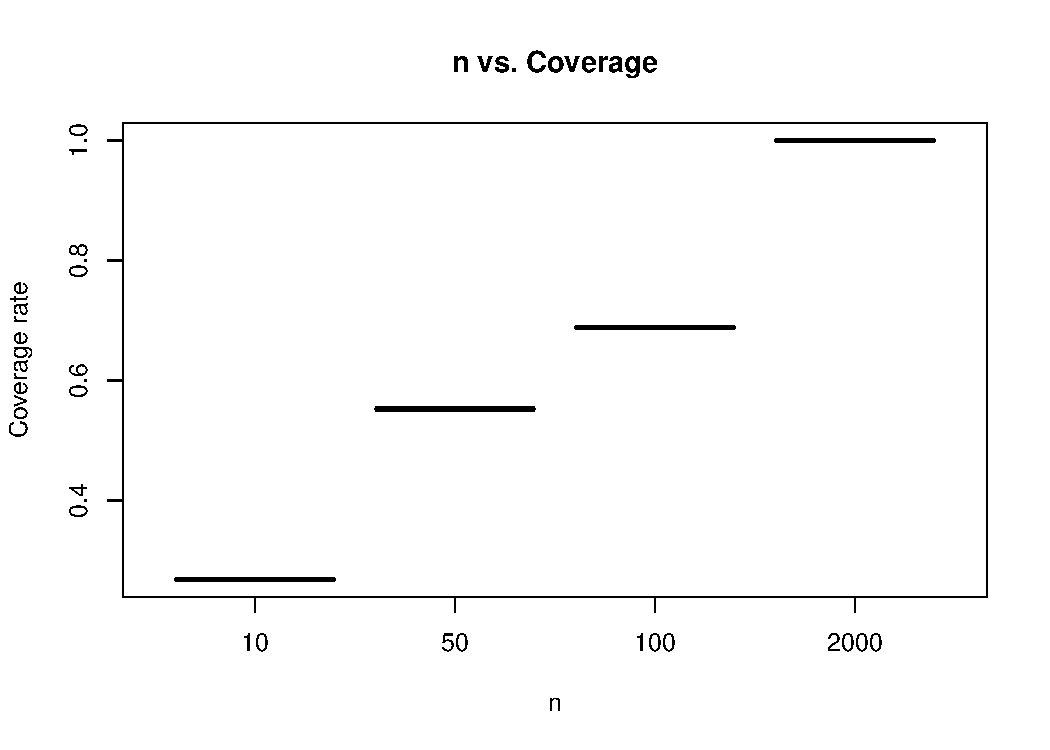
\includegraphics[scale=0.54]{ch4_4.pdf}
\end{figure}

\newpage\noindent
(c) Investigating the relationship between $n$ and the interval length:
$2|\hat{p} - p|$. When does it become smaller than 0.05? According to the simulation
results, that happens roughly when $n$ passes 200, based on our 1000-per-$n$ simulation.
\begin{lstlisting}[style=RSyntax, title=R]
# 4.4(c): Plotting length of interval
IntervalLength <- function(sim) {
    N = ncol(sim); NSIM = nrow(sim)
    intLength = rep(0, NSIM)
    for (i in 1:NSIM) {
        mn = mean(sim[i, 1:N])
        intLength[i] = 2*abs(0.4 - mn) 
    } 
    print(mean(intLength))
} 
> IntervalLength(bsim10)
[1] 0.2408
> IntervalLength(bsim50)
[1] 0.10572
> IntervalLength(bsim100)
[1] 0.077
> IntervalLength(bsim200)
[1] 0.0547
> IntervalLength(bsim300)
[1] 0.04543333
> IntervalLength(bsim2000)
[1] 0.017746
\end{lstlisting}
\begin{figure}[H]
    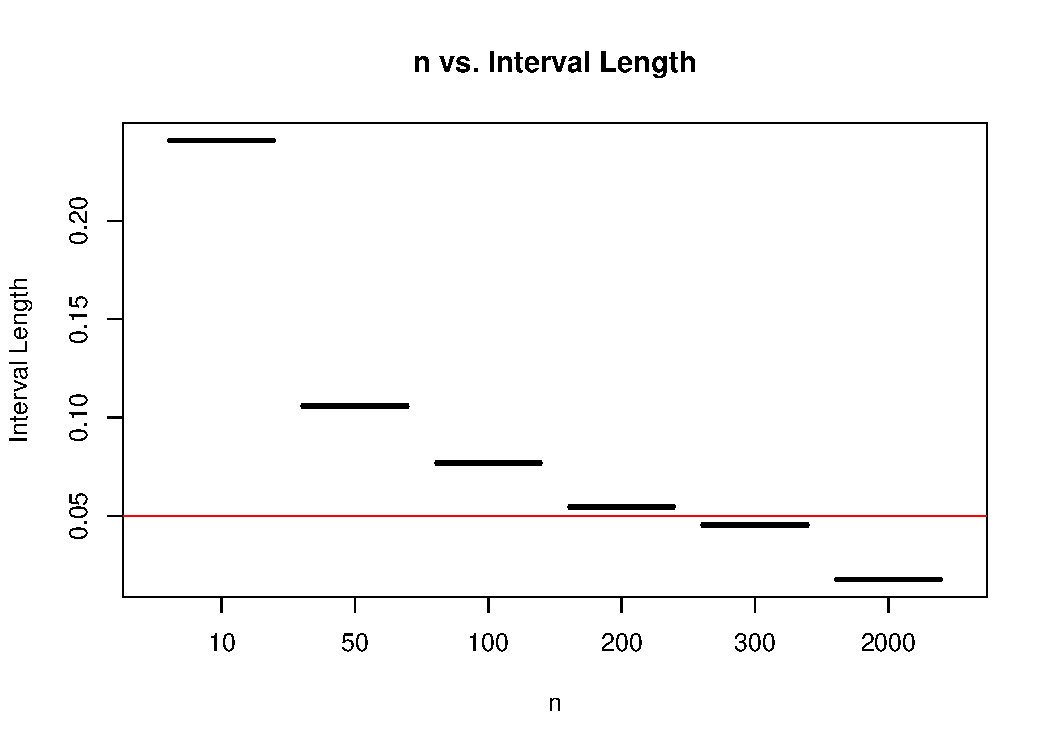
\includegraphics[scale=0.7]{ch4_4b.pdf}
\end{figure}

\newpage\noindent
%%%%%%%%%%%%%%%%%%%%%%%%%%%%%%%%%%%%%%%%%%%%%%%%%%%%%%%%%%%%%%%%%%%%%%%%%%%%%%%
\textbf{4.5} - Theorem 4.7: Mill's Inequality\\  % PDF page 68
Let $Z\sim N(0,1)$ and $t>0$. Then,
$$
\P(|Z| > t) \leq \sqrt{\frac{2}{\pi}}\cdot\frac{e^{-t^2/2}}{t}.
$$
\textsc{Proof}. From the hint, we can use the symmetry property of the normal
distribution, and when $t > 0$:
$$
\P(|Z| > t) = 2\P(Z > t)
\imp
\frac{1}{2}\P(|Z| > t) = \P(Z > t)
\imp
\frac{t}{2}\P(|Z| > t) = t\P(Z > t)
$$
As laid out in the proof of the Markov inequality, we get:
$$
\frac{t}{2}\P(|Z| > t) = t\P(Z > t) = t\int_t^\infty f(x)dx \leq \int_t^\infty xf(x)dx = I
$$
Calculating the integral $I$:
$$
I = \int_t^\infty xf(x)dx =
\frac{1}{\sqrt{2\pi}}\int_t^\infty x\cdot e^{-x^2/2}dx =
\frac{1}{\sqrt{2\pi}}\big[-e^{-x^2/2}\big]_t^\infty = \frac{1}{\sqrt{2\pi}}\Big(0 - (-e^{-t^2/2})\Big)
= \frac{1}{\sqrt{2\pi}}e^{-t^2/2}
$$
Collecting our findings:
$$
\frac{t}{2}\P(|Z| > t) \leq \frac{1}{\sqrt{2\pi}}e^{-t^2/2}
\imp
\P(|Z| > t) \leq \sqrt{\frac{2}{\pi}}\frac{e^{-t^2/2}}{t}
$$
which concludes the proof.\qed

\medskip\noindent
An additional note on the fraction manipulation.
$$
\frac{2}{\sqrt{2\pi}} = \frac{\sqrt{2}\sqrt{2}}{\sqrt{2}\sqrt{\pi}} = \frac{\sqrt{2}}{\sqrt{\pi}} = \sqrt{\frac{2}{\pi}}
$$


\bigskip\noindent
%%%%%%%%%%%%%%%%%%%%%%%%%%%%%%%%%%%%%%%%%%%%%%%%%%%%%%%%%%%%%%%%%%%%%%%%%%%%%%%
\textbf{4.6}\\  % PDF page 68
Let $Z\sim N(0,1)$. We simulate the probability that $\P(|Z| > t)$ and plot the results.
See code and plot on next page.

We will also include the Markov bounds. Since the Markov inequality only applies to
nonnegative random variables, we use it on $|Z|$. Finding $\E[|Z|]$ by using that
the standard normal distribution is symmetric, so we multiply the expected value for
$\E[Z > 0]$ by 2.
\begin{align*}
    \E[|Z|] &= 2\left(\frac{1}{\sqrt{2\pi}}\int_0^\infty x\cdot e^{-x^2/2}dx \right) \\
    &= \sqrt{\frac{2}{\pi}}\Big[-e^{-x^2/2}\Big]_0^\infty \\
    &= \sqrt{\frac{2}{\pi}}\Big(0 - ( - 1)\Big) \\
    &= \sqrt{\frac{2}{\pi}}
\end{align*}
(This can easily be verified numerically).

\newpage\noindent
\begin{lstlisting}[style=RSyntax, title=R]
# Plotting P(Z > t) as a function of t
Z = rnorm(1000000)
t = 1:2000/400 # t goes from 0 to 5
P_Zgt = rep(0, length(t))

for (i in 1:length(t)) {
    P_Zgt[i] = sum(abs(Z) > t[i])
} 
plot(t, P_Zgt/1e6, type="l",
     main="P(|Z|>t) for t in (0,5)")
\end{lstlisting}
Results from plot, when including bounds for the Markov and Hill inequalities:\\
\begin{figure}[H]
    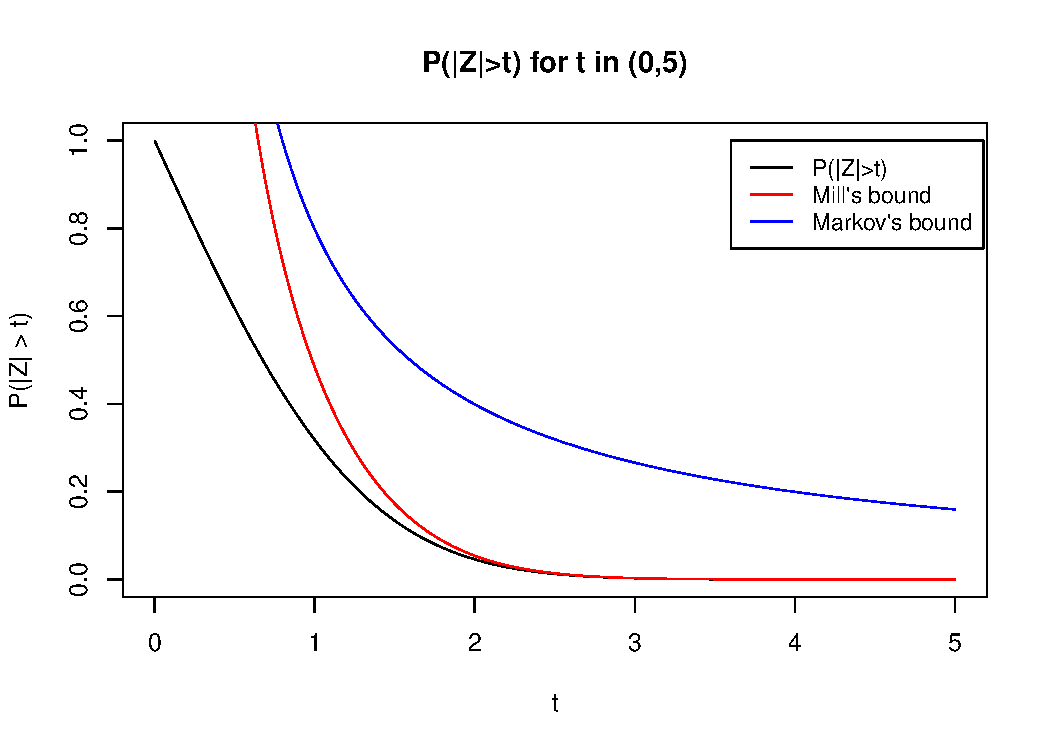
\includegraphics[scale=0.85]{ch4_6.pdf}
\end{figure}
The Markov inequality gives a very lose bound, but as we can see the Mill inequality
gives a bound that really hugs the $\P(|Z| > z)$ curve.

\newpage\noindent
%%%%%%%%%%%%%%%%%%%%%%%%%%%%%%%%%%%%%%%%%%%%%%%%%%%%%%%%%%%%%%%%%%%%%%%%%%%%%%%
\textbf{4.7}\\  % PDF page 68
Let $X_1,\ldots, X_n \sim N(0,1)$. Bound $\P(|\bar{X}| > t)$ using Mill's inequality,
where $\bar{X} = n^{-1}\sum_{i=1}^n X_i$ and compare to Chebyshev's bound.

We begin by applying the Chebyshev's inequality. The sampling distribution of $\bar{X}$
gives $\E[\bar{X}] = 0$ and $\V(\bar{X}) = \sigma^2/n = 1/n$. 
$$
\P(|\bar{X}| > t) = \P(|\bar{X} - \mu| > t) \leq \frac{\sigma^2}{t^2} = \frac{1}{nt^2}
$$
Now, the variable $\bar{X}$ no longer has a standard normal distribution, as we noted above.
We have $\bar{X} \sim N(0, 1/n)$. But we can do the following, since we only require $t > 0$:
\begin{align*}
    \P(|X| > t) &= \P(|0 + (1/n)Z| > t) \\
    &= \P(1/n|Z| > t)\\
    &= \P(|Z| > nt)
\end{align*}
So, by defining $k=nt > 0$, we get:
$$
\P(|X|>t) = \P(|Z| > k) \leq
\sqrt{\frac{2}{\pi}}\frac{e^{-k^2/2}}{k} =
\sqrt{\frac{2}{\pi}}\frac{e^{-(nt)^2/2}}{nt}
$$
No particular observations, except that we can note Hill's inequality relies on the square
of $n$, while Chebyshev's bound only uses $n$. By taking the limit and applying L'Hôpital's
rule, we can easily see that Hill's bound will be smaller as $n$ grows.









\begin{comment}

\bigskip\noindent
%%%%%%%%%%%%%%%%%%%%%%%%%%%%%%%%%%%%%%%%%%%%%%%%%%%%%%%%%%%%%%%%%%%%%%%%%%%%%%%
\textbf{4.X}\\  % PDF page 68


\begin{align*}
    A &= B
\end{align*}


\begin{equation*}
    A = B
    \tag*{\qed}
\end{equation*}


\begin{lstlisting}[style=RSyntax, title=R]
# Code
\end{lstlisting}

\begin{verbatim}
# Output
\end{verbatim}






%%%%%%%%%%%%%%%%%%%%%%%%%%%%%%%%%%%%%%%%%%% Minipages x 2
\begin{figure}[H]
    \begin{minipage}{0.5\textwidth}
        % MINIPAGE 1
    \end{minipage}
    \begin{minipage}{0.5\textwidth}
        % MINIPAGE 2
    \end{minipage}
\end{figure}

%%%%%%%%%%%%%%%%%%%%%%%%%%%%%%%%%%%%%%%%%%% Two R images
\begin{figure}[H]
    \begin{minipage}{0.5\textwidth}
    \begin{center}
        \begin{figure}[H]
            \includegraphics[scale=0.7]{IMG1.pdf}
        \end{figure}
    \end{center}
    \end{minipage}
    \begin{minipage}{0.5\textwidth}
    \begin{center}
        \begin{figure}[H]
            \includegraphics[scale=0.7]{IMG2.pdf}
        \end{figure}
    \end{center}
    \end{minipage}
\end{figure}


%%%%%%%%%%%%%%%%%%%%%%%%%%%%%%%%%%%%%%%%%%% Two TikZ images
%%% Tikz Image - side by side
\begin{figure}
    \begin{minipage}[0.5\textwidth]
\begin{tikzpicture}
    \begin{axis}[
        width=\textwidth,
        axis lines = left,
        ymin = -0.002,
        ymax = 2.1,
        xlabel = $z$,
        ylabel = {$f_Z(z)$},
    ]
    %Section 1
    \addplot [
        domain=0:1, 
        samples=10, 
        color=blue,
        style=ultra thick,
    ]
    {2 - 2*x};
    \end{axis}
\end{tikzpicture}
    \end{minipage}
    \begin{minipage}[0.5\textwidth]
\begin{tikzpicture}
    \begin{axis}[
        width=\textwidth,
        axis lines = left,
        ymin = -0.002,
        ymax = 2.1,
        xlabel = $z$,
        ylabel = {$f_Z(z)$},
    ]
    %Section 1
    \addplot [
        domain=0:1, 
        samples=10, 
        color=blue,
        style=ultra thick,
    ]
    {2 - 2*x};
    \end{axis}
\end{tikzpicture}
    \end{minipage}
\end{figure}
    
\end{comment}